\chapter{Аналитический раздел}

\section{Игра <<Pinball для двух игроков>>}
Игра <<Pinball для двух игроков>> написана на языке C++ с помощью фреймворка cocos2d.

Cocos2d — кросс-платформенный фреймворк, используемый для разработки интерактивных приложений и игр (преимущественно для мобильных устройств). Является открытым программным обеспечением. \cite{wiki-cocos}

Cocos2d-x появился в 2010 году, это проект с открытым исходным кодом, распространяющейся под лицензией MIT. Cocos2d-x позволяет писать на таких языках как C++, Lua и Javascript. Cocos2d-x быстрый, простой и обладает большими возможностями. В настоящее время много игр, написанных с помощью этого фреймворка, находятся в топе AppStore и Google Play. \cite{habrahabr-cocos}

\begin{figure}[h]
  \centering
  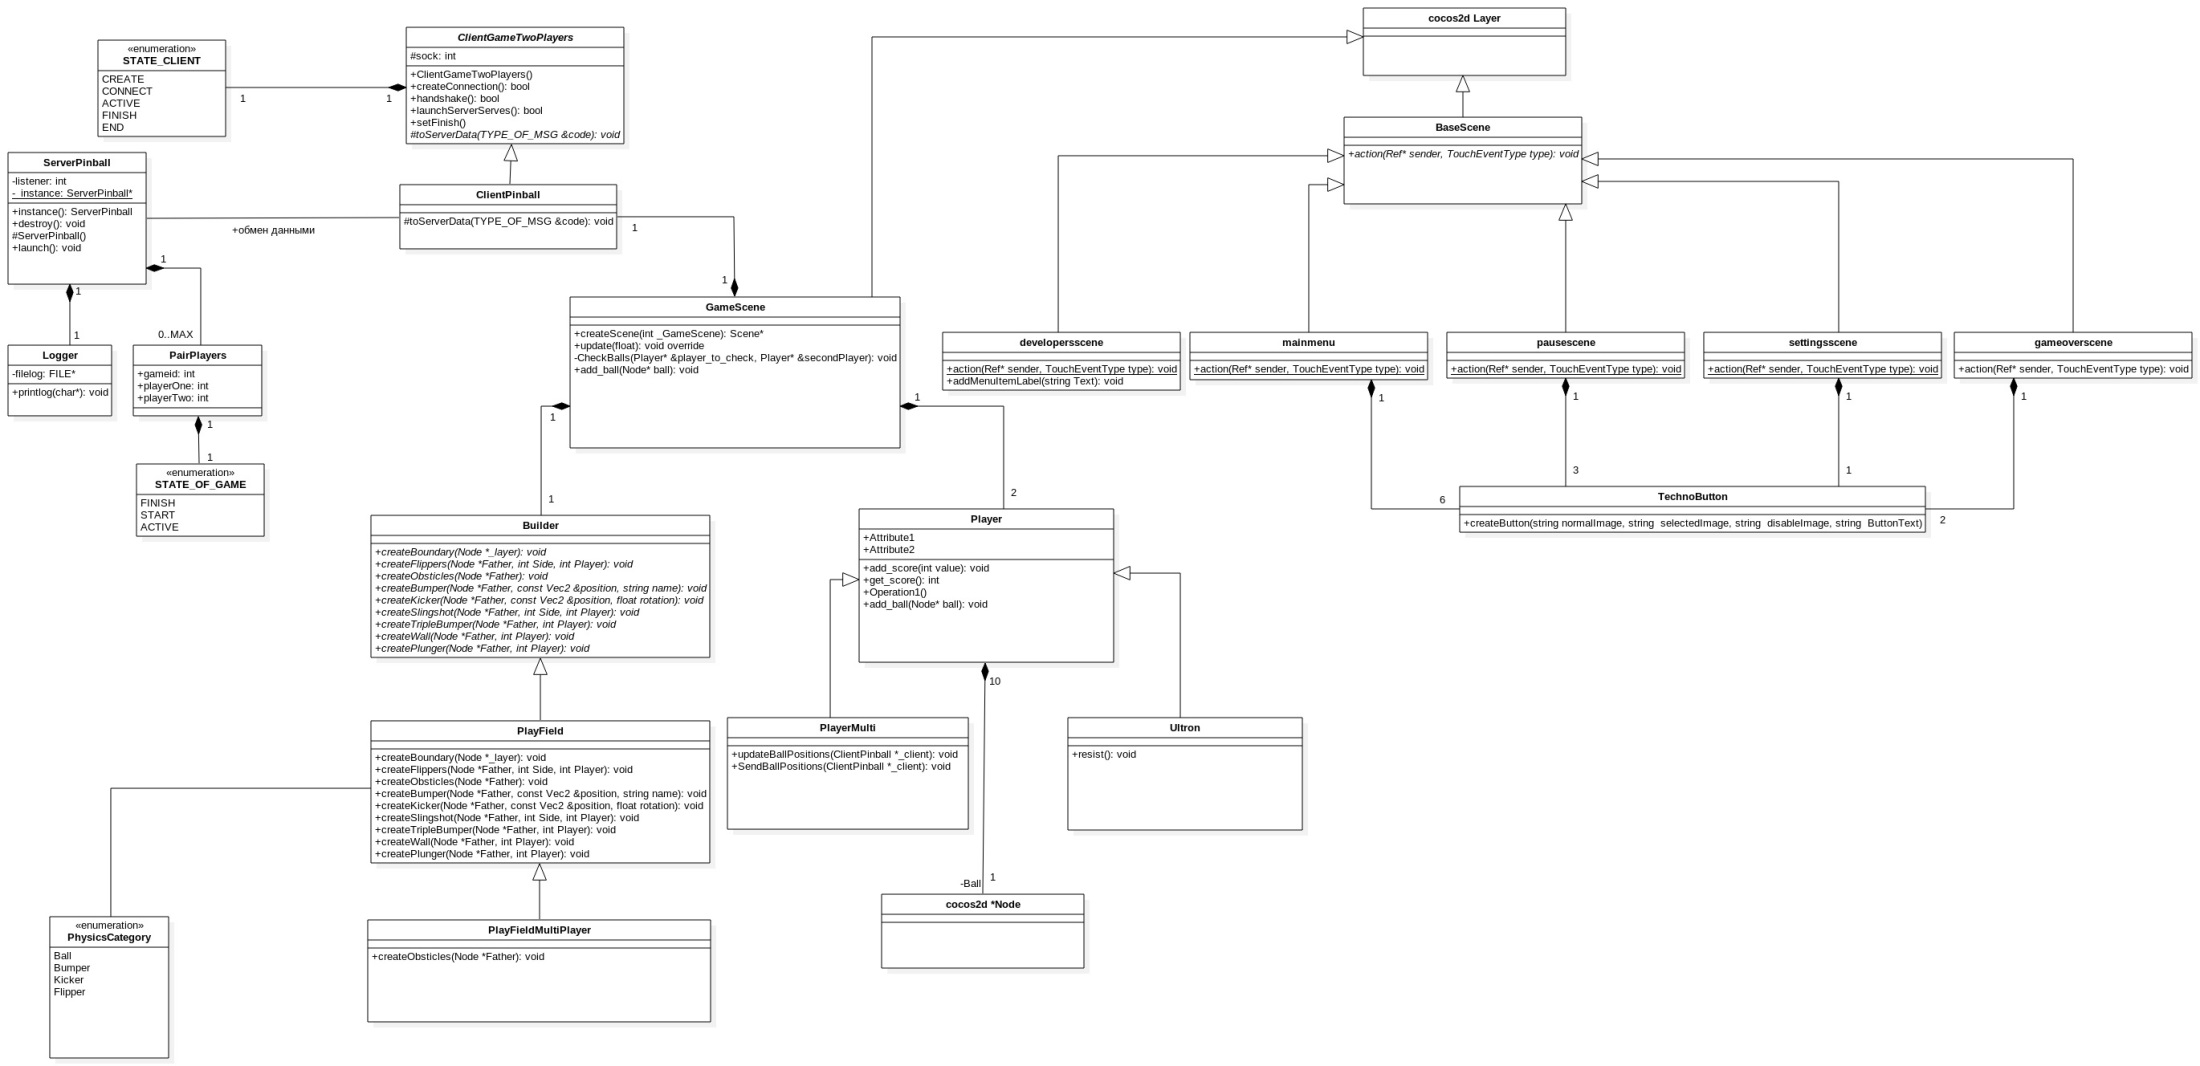
\includegraphics[width=\textwidth]{all-diag.png}
  \caption{Диаграмма классов игры.}
\end{figure}

\section{Gameplay игры}

Игра <<Pinball для двух игроков>> имеет 2 режима работы:
\begin{enumerate}
\item Два пользователя на одной клавиатуре.
\item Пользователь против бота.
\end{enumerate}

На рисунке ~\ref{image:gameplay} показан gameplay игры. Экран игры разбит на два поля. У каждого игрока - своё поле для игры в Pinball. Взаимодейсвтие игроков заключается в перебрасывании шаров через отверстие в стене, разделяющее два поля. На рисунке ~\ref{image:gameplay2} показан момент перелета шара от одно игрока к другому. Поражение наступит либо при утере 5 шаров, либо при отставании в счете от соперника более чем на 12~000~000 очков.

\begin{figure}
  \centering
  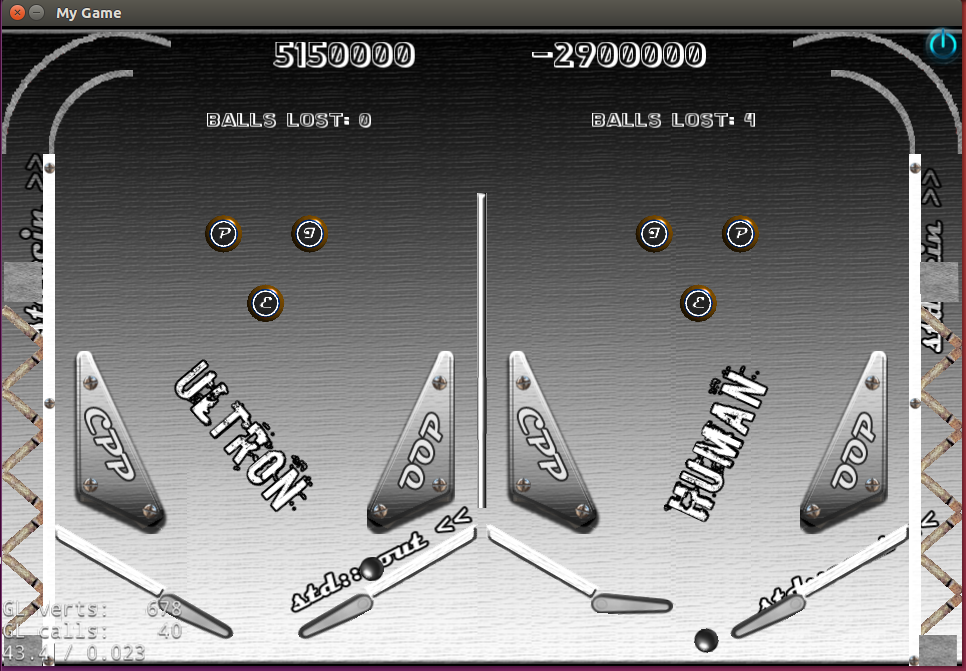
\includegraphics[scale=0.5]{gameplay.png}
  \caption{Gameplay игры.}
  \label{image:gameplay}
\end{figure}

\begin{figure}
  \centering
  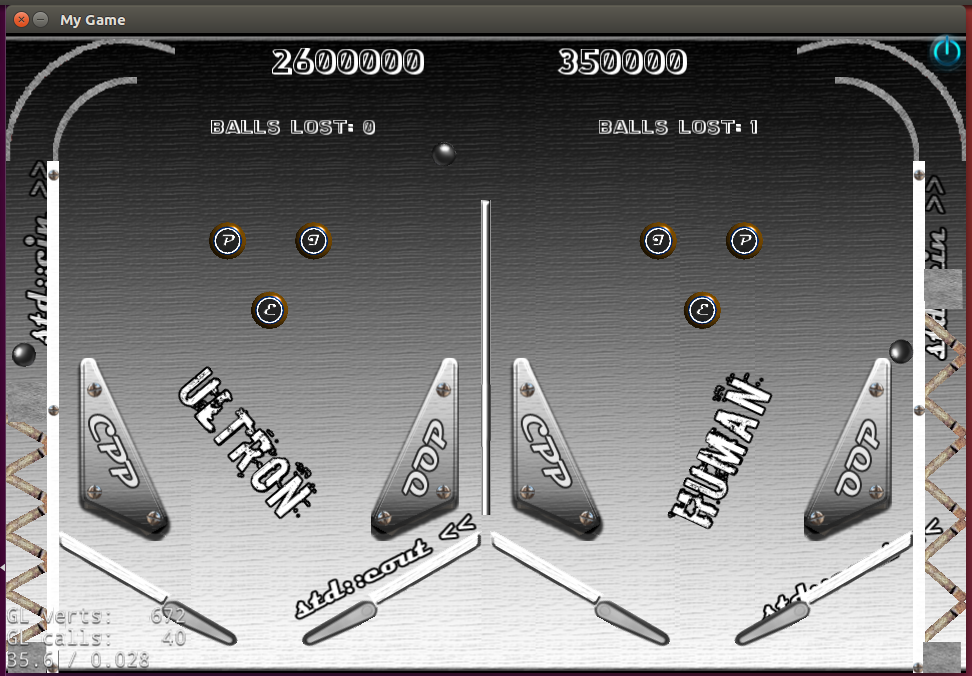
\includegraphics[scale=0.5]{gameplay2.png}
  \caption{Перелет шара.}
  \label{image:gameplay2}
\end{figure}

\section{Передаваемые данные}

Для того, чтобы создать сетевой мультиплеер для данной игры необходимо изучить, какие данные необходимо передавать между клиентами. Между двумя игроками будут передаваться сведения о следующих объектах:
\begin{enumerate}
\item шар;
\item пружина;
\item рычаг;
\item игрок.
\end{enumerate}

В связи со спецификой игры, для каждого объекта будут передавться следующие данные:
\begin{enumerate}
\item шар:
	\begin{enumerate}
	\item координата X;
	\item координата Y;
	\item скорость по X;
	\item скорость по Y;
	\item угол поворота.
	\end{enumerate}	
\item пружина:
	\begin{enumerate}
	\item координата;
	\end{enumerate}
\item рычаг:
	\begin{enumerate}
	\item какой рычаг (левый или правый);
	\item флаг активации;
	\end{enumerate}
\item игрок:
	\begin{enumerate}
	\item счет;
	\item имя;
	\end{enumerate}
\end{enumerate}

\section{Требования к серверу}

При разработке сервера игры необходимо учесть следующие требования:
\begin{enumerate}
\item возможность одновременной игры более 1 пары игроков;
\item поиск соперника происходит простым ожиданием первого подключившегося игрока;
\item запись лога всех событий в файл с числом и временем запуска сервера.
\end{enumerate}

